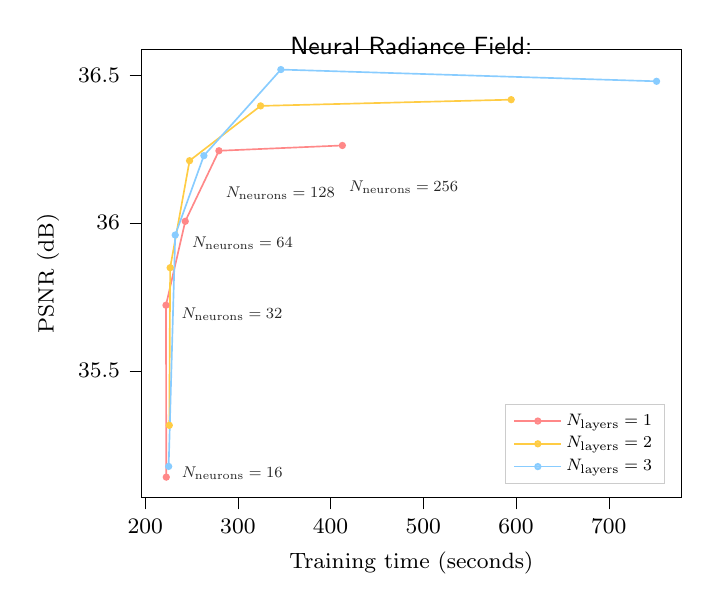
\begin{tikzpicture}
\tikzstyle{every node}=[font=\footnotesize]


\definecolor{color0}{rgb}{1,0.533333333333333,0.533333333333333}
\definecolor{color1}{rgb}{1,0.8,0.266666666666667}
\definecolor{color2}{rgb}{0.533333333333333,0.8,1}

\begin{axis}[
legend cell align={left},
legend style={
  fill opacity=0.8,
  draw opacity=1,
  text opacity=1,
  at={(0.97,0.03)},
  anchor=south east,
  draw=white!80!black,
  nodes={scale=0.75, transform shape}
},
tick align=outside,
tick pos=left,
title={{\small \sffamily Neural Radiance Field: \sceneLego}},
title style={at={(0.5,0.93)}},
x grid style={white!69.0196078431373!black},
xlabel={Training time (seconds)},
xmin=195.985047805309, xmax=777.987818491459,
xtick style={color=black},
y grid style={white!69.0196078431373!black},
ylabel={PSNR (dB)},
ymin=35.0719980023238, ymax=36.5867545285986,
ytick style={color=black}
]
\addplot [semithick, color0, mark=*, mark size=1, mark options={solid}]
table {%
222.772186994553 35.1408505716999
222.439719200134 35.7217079502554
243.241554498672 36.0052576758842
279.554010391235 36.243565324869
412.660806894302 36.26144806088
};
\addlegendentry{$N_\mathrm{layers}=1$}
\addplot [semithick, color1, mark=*, mark size=1, mark options={solid}]
table {%
226.028396368027 35.3159206831678
226.953627824783 35.8484963859825
247.891683340073 36.2100016867744
324.485737800598 36.3951691878594
594.732287883759 36.4161708629578
};
\addlegendentry{$N_\mathrm{layers}=2$}
\addplot [semithick, color2, mark=*, mark size=1, mark options={solid}]
table {%
225.336002111435 35.1770899611643
232.406004190445 35.9588434010099
263.312616586685 36.2269686218852
346.350400924683 36.5179019592225
751.533147096634 36.4782679346175
};
\addlegendentry{$N_\mathrm{layers}=3$}
\draw (axis cs:232.26661798954,35.1408505716999) node[
  scale=0.7,
  anchor=base west,
  text=white!15!black,
  rotate=0.0
]{$N_\mathrm{neurons} = 16$};
\draw (axis cs:231.934150195122,35.6768840506882) node[
  scale=0.7,
  anchor=base west,
  text=white!15!black,
  rotate=0.0
]{$N_\mathrm{neurons} = 32$};
\draw (axis cs:243.241554498672,35.9156098767498) node[
  scale=0.7,
  anchor=base west,
  text=white!15!black,
  rotate=0.0
]{$N_\mathrm{neurons} = 64$};
\draw (axis cs:279.554010391235,36.0866816763838) node[
  scale=0.7,
  anchor=base west,
  text=white!15!black,
  rotate=0.0
]{$N_\mathrm{neurons} = 128$};
\draw (axis cs:412.660806894302,36.1045644123948) node[
  scale=0.7,
  anchor=base west,
  text=white!15!black,
  rotate=0.0
]{$N_\mathrm{neurons} = 256$};
\end{axis}

\end{tikzpicture}
